 \documentclass[12pt,english]{article}
\usepackage[utf8]{inputenc}
\markright{Pearse et al.\hfill Assessing the Effects Imputation on ED Values\hfill}
\usepackage{geometry}
\geometry{verbose,letterpaper,tmargin=2.54cm,bmargin=2.54cm,lmargin=2.54cm,rmargin=2.54cm}
%\geometry{verbose,letterpaper,tmargin=.1cm,bmargin=.1cm,lmargin=.1cm,rmargin=.1cm}
\usepackage{graphicx}
\DeclareGraphicsExtensions{.pdf,.png,.jpg}
\usepackage{amssymb,amsmath}
\usepackage{epstopdf}
\usepackage{tocbibind}
\usepackage[toc,page]{appendix}
\usepackage{supertabular}
\DeclareGraphicsRule{.tif}{png}{.png}{`convert #1 `dirname #1`/`basename #1 .tif`.png}
\usepackage{url}
\usepackage{subcaption}
\usepackage{caption}
\usepackage[super]{nth}
\usepackage{lineno} \linenumbers
\usepackage[doublespacing]{setspace}
\usepackage[parfill]{parskip}
\setlength{\parindent}{0pt}
\usepackage[citestyle=authoryear,bibstyle=authoryear,sorting=nyt,maxcitenames=2,maxbibnames=10,minbibnames=6,doi=false,url=false,isbn=false,firstinits=true,uniquename=false,uniquelist=false]{biblatex}
\bibliography{edge_sims}
\renewbibmacro*{name:andothers}{% Based on name:andothers from biblatex.def
  \ifboolexpr{
    test {\ifnumequal{\value{listcount}}{\value{liststop}}}
    and
    test \ifmorenames
  }
    {\ifnumgreater{\value{liststop}}{1}
       {\finalandcomma}
       {}%
     \andothersdelim\bibstring[]{andothers}}
    {}}
\renewcommand*{\finalnamedelim}{%
  \ifnumgreater{\value{liststop}}{2}{\finalandcomma}{}%
  \addspace\&\space}
\renewbibmacro{in:}{}
\AtEveryBibitem{%
  \clearfield{day}%
  \clearfield{month}%
  \clearfield{endday}%
  \clearfield{endmonth}%
}
\DeclareFieldFormat[article]{citetitle}{#1}
\DeclareFieldFormat[article]{title}{#1}
\DeclareFieldFormat[article]{pages}{#1}
\DeclareNameAlias{sortname}{last-first}

\usepackage{changes}
\setdeletedmarkup{\textcolor{red}{\sout{#1}}}

\begin{document}
\setlength{\parindent}{0pt}
\section*{Title page}

\textbf{Article title}: A simulation of the effect of phylogenetic
missing species and their imputation on evolutionary distinctiveness
scores

\textbf{Running head}: Evolutionary distinctiveness and missing
species

\textbf{Authors:} K.\ Bodie Weedop$^{1}$, Arne \O. Mooers$^2$,
Caroline M.\ Tucker$^3$, and William D.\ Pearse$^{1}$\

$^1$ Department of Biology \& Ecology Center, Utah State University,
5305 Old Main Hill, Logan UT, 84322

$^2$Department of Biological Sciences, Simon Fraser University,
Burnaby, British Columbia, Canada

$^3$Department of Biology, University of North Carolina--Chapel Hill

$^*$To whom correspondence should be addressed:
\url{will.pearse@usu.edu}

\textbf{Word-count}: 5680 (abstract, main text, acknowledgments, and
  references)

\clearpage
\section*{Abstract}

As global extinction rates have risen, conservation biologists are
increasingly focusing on how best to allocate their limited time and
money to save as much diversity as possible. Increasingly, conservation
effort is being allocated on the basis not just of species'
endangerment, but also the evolutionary history (and so phylogenetic
diversity) that they represent. Metrics such as EDGE (Evolutionary
Distinct and Globally Endangered) have been successfully used to set
conservation priorities for a number of taxa, such as mammals, birds,
corals, and sharks.  Each of these applications of EDGE has required
some form of correction for species whose position within the tree of
life are unknown. Perhaps the most advanced of these corrections is
phylogenetic imputation, but to date there has been no systematic
assessment of the impact of both missing species and imputation to
correct for them. Here we perform such a systematic assessment,
simulating the random loss of species from a phylogeny, the imputation
of the position of those species, and measure the impact each of these
processes has on the data underlying EDGE scores. We find that EDGE
ranking is remarkably robust to missing species, and that phylogenetic
imputation, while unbiased, is not accurate in reconstructing species'
true evolutionary distinctiveness. On the basis of these results, we
provide clear guidance for EDGE scoring in the face of phylogenetic
uncertainty.

\textbf{Keywords}: conservation prioritization, evolutionary
distinctiveness, EDGE, phylogenetic imputation.

\clearpage
\section*{Introduction}

Evidence from the fossil record and present-day studies argue we are in the
midst of, or entering, a sixth mass extinction \autocite{Barnosky2011,
Ceballos2015}, such that more species than ever are declining and/or in danger
of extinction across a range of environments \autocite{Wake2008,Thomas2004}.
Habitat destruction \autocite{Brooks2002}, invasive species
\autocite{Molnar2008}, climate change \autocite{Pounds2006}, and disease
\autocite{Lips2006} are some of the leading causes of species declines globally.
Conservation biologists seek to reduce these detrimental effects on species
populations, but in reality they have limited resources with which to do so.
This challenge, termed the ``Noah's Ark problem'' \autocite{Weitzman1998}, has
driven conservation biologists to prioritize, or triage, their resource allocation
\autocite{Bottrill2008}.

Conservation triage, like all sound decision-making, requires some metric that
quantifies the urgency for conservation of a set of species. By using such a
metric, researchers are able to avoid biasing the allocation of time and
resources for conservation, and can make their conservation goals more explicit.
One such triage strategies which has been widely used is the EDGE metric
\autocite[Evolutionary Distinction and Globally Endangered;][]{Isaac2007}. This
method prioritizes species according to two criteria: Evolutionary
Distinctiveness (ED) and Global Endangerment (GE). ED measures relative
contributions to phylogenetic diversity made by each species within a particular
clade \autocite{Isaac2007}, assigning each branch length equally to all its
subtending species. GE values are quantified by assigning numerical values to
each of the World Conservation Union (IUCN) Red List Categories. As species
become increasingly threatened and are placed into more concerning categories
(\emph{e.g.}, from Vulnerable to Endangered), the GE numerical value increases.
Thus a species' EDGE score is intended to equally reflect a species' evolutionary
distinctiveness and conservation status \autocite[even if it does not always in practice; see][]{Pearse2015}.

The EDGE approach was never intended to be a purely academic, and is now
the basis of the global EDGE of Existence Program
(\url{http://www.edgeofexistence.org/}). While EDGE was originally used to
prioritize global mammals, it has subsequently been applied to a number of
species groups, including amphibians \autocite{Isaac2012}, birds 
\autocite{Jetz2014}, corals \autocite{Curnick2015}, and sharks
\autocite{Stein2018}. A number of similar metrics  have been developed, each
prioritizing and emphasizing subtly different things, such as the expected
contribution of each species to overall phylogenetic diversity
\autocite[HEDGE;][]{Steel2007}, our uncertainty over a species' future
\autocite[EDAM;][]{Pearse2015}, and the complementarity of a set of species
\autocite{Faith2008,Jensen2016}. Thus the development of EDGE-like metrics has
matched progress with other fields of conservation biology, where the likelihood
of success in conservation \autocite{Wilson2007, Mcbride2007}, relative cost of
certain interventions \autocite{Naidoo2006}, and complementarity of
interventions \autocite{Pressey1993, Myers2000} have also been considered.
Critically, EDGE has formed the basis of a successful program that
quantitatively prioritizes conservation, providing actionable insights into how
to focus conservation effort in the face of uncertainty about species'
attributes. EDGE's success proves that phylogenetic conservation prioritization
metrics can be used by conservation biologists and policy makers, and that they
are popular with the public. Nonetheless, almost every application of an
EDGE-like approach has had to deal with the uncertainty presented by missing
species data.

IUCN has given guidance that any available contextual data should be used to
assign some threat status to species which are classified as Data Deficient
\autocite{Iucn2001, Iucn2008}. A number of studies have been done
showing how to follow this guidance and assign threat categories to Data
Deficient species and reduce the uncertainty in GE \autocite{Good2006,
Butchart2010, Morais2013}. The problem, however, is arguably more complex for
species whose phylogenetic position is unknown. Species of conservation concern
are almost by definition rare, and so we frequently lack sufficient DNA (or even
morphological) data to place them with certainty on a phylogeny. In the face of
such essentially unavoidable uncertainty, conservation biologists have worked
hard to overcome data limitations. In most empirical EDGE lists taxonomic
information, rather than sequence data alone, is used to locate species in the
tree of life \autocite{Isaac2007,Collen2011,Isaac2012,Jetz2014,Curnick2015,
Gumbs2017,Stein2018}. By using taxonomic information, researchers are
able to produce fully resolved phylogenies using model-based imputation
\autocite{Kuhn2011, Thomas2013}. Yet, to our knowledge, there has yet to be a
systematic study of the effect of such imputation on species' EDGE scores,
unlike in other aspects of comparative biology \autocite{Rabosky2014}. Indeed,
there is no clear guidance as to the size of the effect of ignoring missing
species on remaining species during prioritization, or the magnitude of error
phylogenetic imputation introduces. As the desire to use ED and phylogenies for
conservation triage grows, the need for such tests and a consensus on how
to resolve cases of phylogenetic uncertainty becomes more urgent.

Here we quantify the effect of missing species on EDGE rankings and assess
whether imputing species is a defensible method for dealing with species missing
phylogenetic data. We do so by simulating the removal of species from simulated
trees in two ways: at random and in a phylogenetically biased manner. By doing
so, we hope to provide two reasonably realistic case-studies of how species
might be expected to be missing from the tree of life. We also assess the extent
to which imputed species' EDGE rankings correlate with their true values. To do
this, we simulate phylogenies, choose clades at random to remove, and then
impute the structure of these clades, all under the same model of
diversification. In so doing, we hope to provide clear guidance as to the
applicability of phylogenetic imputation as a solution for species missing
phylogenetic data. From our results, we argue that species' ED values are
remarkably robust to the loss of species, and that phylogenetic imputation does
not reliably reconstruct the true ranking of species.

\section*{Methods}

Here we use a simulation approach to test the effect of removing and imputing
species on a phylogeny on species' ED (Evolutionary Distinctiveness) scores.
Since empirical studies do not (to our knowledge) impute GE (Global
Endangerment) scores for species, instead relying on the IUCN's proposal to
assign Data Deficient species as threatened or otherwise based upon any
available evidence, we focus solely on phylogenetic imputation. EDGE is the
product of both ED and GE \autocite[see]{Isaac2007}, thus perfectly accurate GE values could still lead to
an imperfect EDGE score if the ED scores were imperfectly calculated.

All simulations and analyses were performed using R \autocite[version
3.4.0;][]{R2017}, and we performed 100 replicate simulations of each parameter
combination . All trees (both starting and imputed) were simulated under a
pure-birth Yule model using the \texttt{sim.bdtree} function under parameters of
in the \texttt{geiger} R package \autocite[under parameters \texttt{b=1} and \texttt{d=0};][]{Pennell2014}. 
This particular model was chosen because it is the simplest model possible:
speciation rates are constant across the entire tree of life and there is no
extinction. We acknowledge that it is possible that more complex and/or
biologically realistic models of diversification could improve the performance
of imputation. However, we suggest that imputation under a simple model that is
identical to that used to simulate the data is a low, and fair, benchmark for a method to
meet. We used \texttt{ed.calc} in the R package \texttt{caper} to calculate
ED values \autocite{Orme2013}. All our analysis code is available online in the supplementary materials and at \url{https://github.com/bweedop/edgeSims}.

\subsection*{The impact of missing species on EDGE scores}
Our first set of simulations assessed the impact of random and
phylogenetically-biased loss of species from a phylogeny on ED scores. Both sets
of simulations were carried out using phylogenies of different sizes (64, 128, 256, 512, 1024, 2048, and 4096 species), removing constant fractions of tips from
the tree (0\%, 1\%, 2\%, ..., 98\%, and 99\%). To simulate randomly missing
species, we used the \texttt{sample} function in R to select the relevant
percentage of species (rounded to the nearest whole number) without replacement.
Thus this randomization did not incorporate phylogenetic structure. To remove
species in a phylogenetically biased manner, we used
\textcite{Felsenstein2005}'s threshold model. First, we simulated a trait under
a constant rate Brownian-motion model ($\sigma^2$=0.5, starting root value = 1).
using the \texttt{sim.char} function in the \texttt{geiger} R package
\autocite{Pennell2014} Species were then removed from the tree if their
simulated trait was in the upper quantile of whatever fraction of species were
to be dropped. For example, if 10\% of species were to be dropped, species
within the upper \nth{10} quantile of character trait values were removed from
the tree. 

We calculated species' ED values before removal of species from the tree and
afterwards. We then correlated the ED scores (using the \texttt{cor} function in
the \texttt{stats} R package) of the species left in the tree with their
original ED values, to measure the effect of species' removal on ED scores. If missing species have no effect upon ED values, we
expect a high, positive coefficient of correlation between the remaining
species' ED scores before and after the other species were removed from the
tree. We outline our approach in figure \ref{conceptual}a.

\begin{figure}[!ht]
  \center
  \begin{subfigure}{0.9\textwidth}
    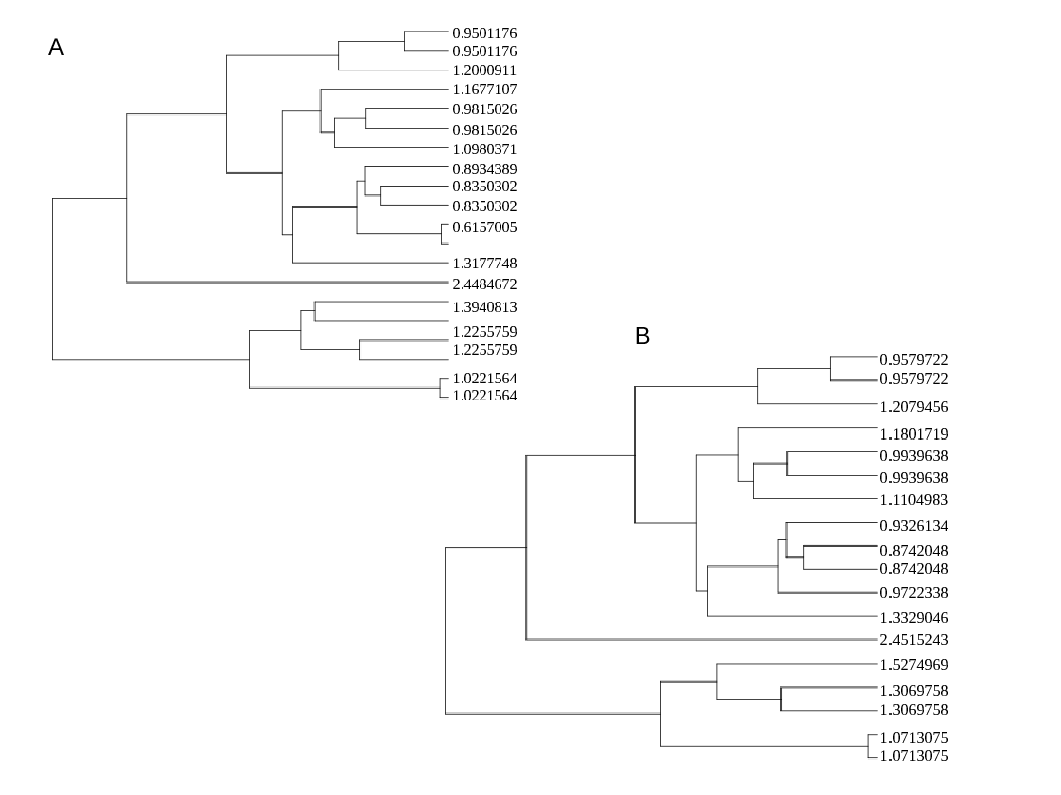
\includegraphics[width=.75\textwidth]{missingSpecies.png}      
    \caption{Simulating missing species}
  \end{subfigure}
  \\
  \begin{subfigure}{0.9\textwidth}
    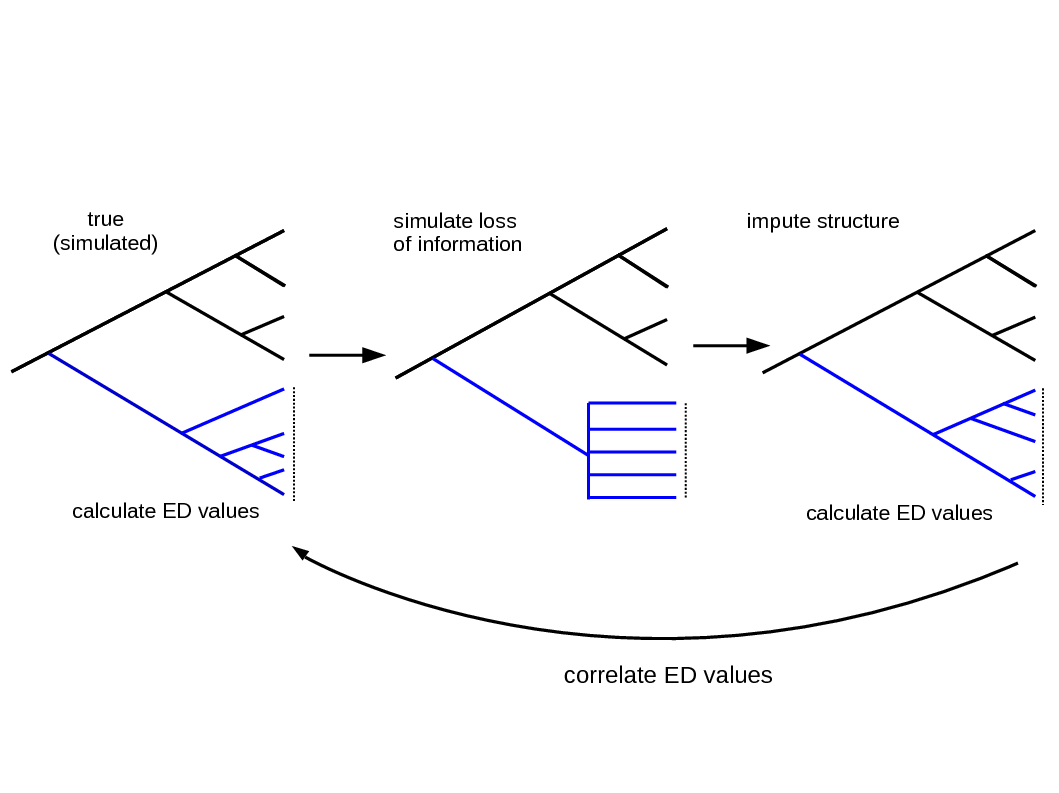
\includegraphics[width=.75\textwidth]{imputeConcept.png}      
    \caption{Simulated imputed species}
  \end{subfigure}
  \caption{\textbf{Conceptual overview of the simulations conducted in
      this study.} In (a), the simulated tree on the left is the true
    tree prior to removal of missing species. On the right is the same
    tree after the removal of missing species. We correlate the ED
    values of the remaining species (indicated with dashed lines) to
    measure the impact of missing species on known species. In (b),
    the simulated tree on the left is the true tree prior to loss of
    information. To the right is each step in the process of
    simulating the imputation of species within the clade highlighted
    with the dashed line. To compare true and imputed ED values, we
    correlate ED values on the full phylogeny and imputed clade.}
  \label{conceptual}
\end{figure}

\subsection*{The impact of phylogenetic imputation on EDGE scores}
We tested the impact of imputing missing species in relatively small clades
(3, 4, ..., 31, and 32 species) from phylogenies of different sizes (64, 128,
256, 512, and 1024 species). We first randomly selected a clade to be removed
from the original tree, simulated a new phylogeny of the same size under the
same pure-birth model used to generate the phylogeny, and placed the newly
simulated clade back where the original clade was removed. If a newly simulated clade were so old that it was not possible to graft it into place, we discarded that clade and simulated another. Thus we imputed each
clade under the model used to generate it: in an empirical study this model
would, itself, have to be inferred but we do not address this additional source
of error here. An overview of our approach is given in figure \ref{conceptual}b.

To assess whether clades, once imputed, had similar ED scores, we
correlated the imputed ED scores against true ED scores. We also
calculated the sum of the absolute change in ranked ED for each
species, which is particularly relevant for EDGE-listing as it is
often the top 100, 200, etc., species on which conservation actions
are targeted. We statistically modeled both these metrics as a
function of a number of potential explanatory variables, specifically:

\begin{itemize}
\item The estimated speciation rate of the original phylogeny
  \autocite[$\lambda$, using the \texttt{yule} function in the R
  package \texttt{ape};][]{Paradis2004}
\item The sum of all phylogenetic branch-lengths in the original phylogeny
  \autocite[essentially Faith's PD;][]{Faith1992}
  \item $\gamma$ in the original phylogeny
  \autocite[using the \texttt{gammatest} function in the R package
  \texttt{phytools};][]{Pybus2000,Revell2012},
\item Colless' index of the original phylogeny \autocite[using the
  \texttt{as.treeshape} function in the R package
  \texttt{apTreeshape};][]{Colless1982,Bortolussi2009}
\item The kurtosis of species' ED values in the original phylogeny
  \autocite[using the \texttt{moments} function in the R package
  \texttt{kurtosis};][]{Komsta2015}
\item The skew of species' ED values in the original phylogeny
  \autocite[using the \texttt{skew} function in the R package
  \texttt{moments};][]{Komsta2015}
\item The total number of species in the original phylogeny
\item The total number of species within the imputed clade
\end{itemize}

Although the expectations of many of these explanatory variables are
known from theory, in each simulation they are expected to vary
somewhat by chance.

\clearpage
\section*{Results}
Under both random and phylogenetically-patterned loss, species' ED
scores are less accurate as more species are removed from the tree
(table \ref{missing_ancova} and figure \ref{randomVsClustered}). ED
values are less robust to phylogenetically-biased, rather than
randomly selected, missing species: if 20\% of species are missing,
the average correlation between true and estimated ED is 0.88 and 0.94
for phylogenetically-biased and random missing species, respectively.

We find no support for a correlation between the imputed and true ED
values for species within imputed clades (figure \ref{imputationTrend}
and table \ref{imputeReg}). We could find no explanatory variables
that significantly predicted variation in this trend (table
\ref{imputeReg}; see also Supplementary Materials), but we do find
evidence that, when imputing larger clades, the variation in
correlation is lesser but remains centered on a mean of zero
correlation (see Supplementary Materials). Imputed rankings of species
within clades are also altered under imputation (figure
\ref{rankingError} and table \ref{impute_model}). This ranking error
increases with the size of the imputed clade and phylogeny (table
\ref{rankingError}), and can affect ranking error within the top 100
and 250 species (see Supplementary Materials). To give an example of
the magnitude of the effect, within a phylogeny of 1024 species, the
members of an imputed clade of 30 species are, on average, $\pm$ 315
rankings from their true rankings.

\begin{figure}[!ht]
  \center
  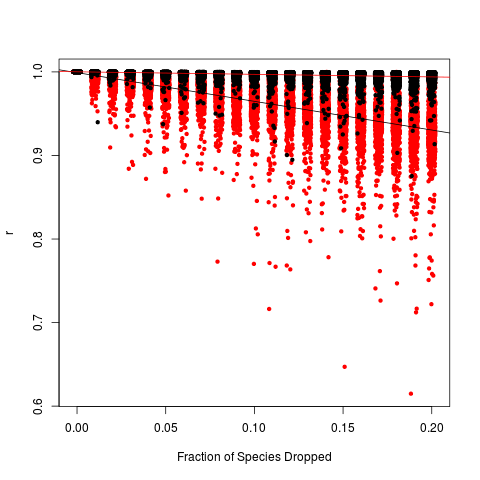
\includegraphics[width=.5\textwidth]{randomVsCluster.png}
  \caption{\textbf{R-values plotted against the fraction of species dropped at
  random versus clustered manner.} The color of data points denote whether
  species were dropped at random (orange; n = 100) or in clustered manner
  (grey; n = 100). The regression lines are demonstrating the relationship when
  species are dropped at random (red) and in a clustered manner (clustered). The
  correlations represent a comparison of the ED values (before and after
  species are dropped) of species which remain on the on the phylogeny after
  other species are dropped.}
  \label{randomVsClustered}
\end{figure}

\begin{table}[ht]
  \centering
  \begin{tabular}{rrrrr}
    \hline
      & Estimate & Std. Error & t value & Pr($>$$|$t$|$) \\
      \hline
      (Intercept) & 1.0315 & 0.0013 & 821.39 & $<$0.0001 \\
      Fraction of Species Dropped & -0.4696 & 0.0020 & -233.16 & $<$0.0001 \\
      Random Treatment & 0.0630 & 0.0018 & 35.47 & $<$0.0001 \\
      Number of Species Overall & 0.0000 & 0.0000 & 7.89 & $<$0.0001 \\
      Fraction of Species Dropped:Random Treatment & -0.2774 & 0.0028 & -97.45 & $<$0.0001 \\
      Random Treatment:Number of Species Overall & 0.0000 & 0.0000 & -4.38 & $<$0.0001 \\
      \hline
    \hline
  \end{tabular}
  \caption{\textbf{ANCOVA model summary describing the effect of
      dropping species on remaining species ED Values.} The fraction
    of species dropped significantly affects the the remaining ED
    values. Dropping the fraction both at random and in clustered
    manner both have negative effects on the remaining ED values
    ($F_{139696, 5}$ = 40350, $R^{2}$ = 0.5908, p$<$0.0001).}
  \label{missing_ancova}
\end{table}

\begin{figure}[!ht]
  \center
  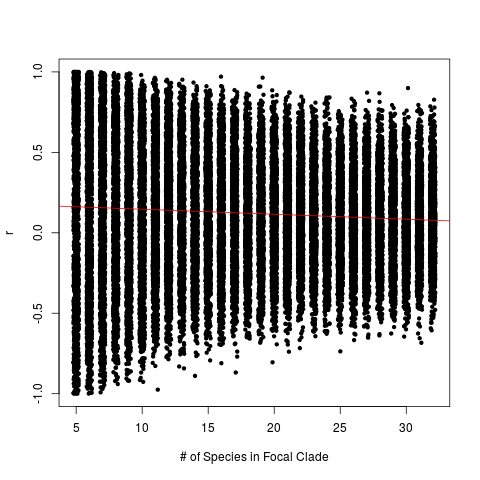
\includegraphics[width=.5\textwidth]{edModel.png}
  \caption{\textbf{R-values plotted against the number of species at focal
  clade.} Each data point denotes a correlative comparison between ED values
  within the focal clades where imputation has occurred. The regression line
  (red) and trend even closer to zero demonstrates the decrease in informative
  value of the imputed ED values. This is reinforced by the visual narrowing of
  r-values around zero.}
  \label{imputationTrend}
\end{figure}

\begin{table}[ht] 
\centering
\begin{tabular}{rrrrr}
  \hline
  & Estimate & Std. Error & t value & Pr($>$$|$t$|$) \\
   \hline
   (Intercept) & 0.1691 & 0.0500 & 3.38 & 0.0007 \\
   Size of Focal Clade & -0.0029 & 0.0002 & -14.15 & 0.0000 \\
   Size of Phylogeny & -0.0001 & 0.0001 & -1.01 & 0.3128 \\
   PD & 0.0001 & 0.0001 & 0.97 & 0.3339 \\
   Lambda & 0.0051 & 0.0492 & 0.10 & 0.9179 \\
   Colless' Index & 0.0020 & 0.0021 & 0.96 & 0.3388 \\
   Skew & 0.0039 & 0.0083 & 0.47 & 0.6409 \\
   Kurtosis & -0.0005 & 0.0008 & -0.64 & 0.5247 \\
   \hline
   \hline
\end{tabular}
\caption{\textbf{Effect of Clade Size on Imputed ED Values.} The
intercept describes that the correlation between the true and imputed values
begins quite low. As the clade size increases, this correlation only tends
toward zero. The total number of species in the full phylogeny along with
measures of the true phylogenetic diversity, lambda, Colless' Index, skew, and
kurtosis show no significant effect. ($F_{47992, 7}$ = 29.38, $R^{2}$ = 0.005,
p$<$0.0001).}
\label{imputeReg}
\end{table}

\begin{figure}[!ht]
  \center
  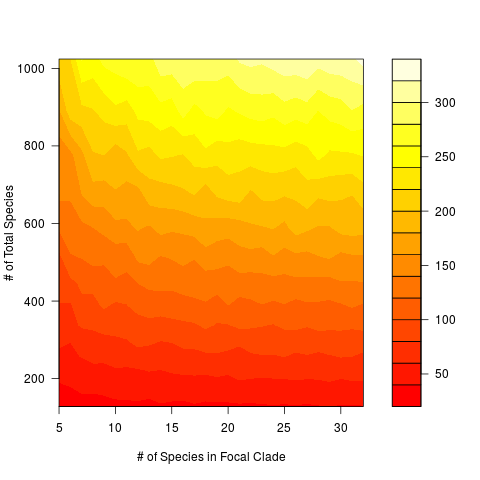
\includegraphics[width=.5\textwidth]{rankingError.png}
  \caption{\textbf{Mean ranking error of species within the focal clade.} The 
  gradient on the right demonstrates average number of positions within the 
  full ranking that focal clade species shifted from their true rank.
  While controlling for the size of the full phylogeny and focal clade, species 
  within the focal clade were, on average, ranked far from the true rank. }
  \label{rankingError}
\end{figure}

\begin{table}[ht]
  \centering
  \begin{tabular}{rrrrr}
    \hline
   & Estimate & Std. Error & t value & Pr($>$$|$t$|$) \\
    \hline
  (Intercept) & -1.6344 & 0.0332 & -49.29 & 0.0001 \\
    Size of Focal Clade & 0.0900 & 0.0010 & 91.22 & 0.0001 \\
    Size of Phylogeny & 0.5179 & 0.0013 & 383.99 & 0.0001 \\
     \hline
     \hline
  \end{tabular}
  \caption{\textbf{Effect of Clade Size and Total Species on Ranking
  Error.} Model demonstrating the relationship between focal clade species
  ranking error and the size of imputed clade and overall phylogeny. Square-root
  transformations have been applied to both ranking error and size of phylogeny.
  Significant increases ranking error are seen when increasing sizes of both the
  imputed clade and phylogeny ($F_{47997, 2}$ = 77890, $R^{2}$ = 0.7644,
  p$<$0.0001).}
\label{impute_model}
  \end{table}

\clearpage
\section*{Discussion}
Phylogeny is increasingly playing a role in conservation prioritization,
decision-making, and policy. A major obstacle to a more widespread adoption of
phylogenetic prioritization methods such as EDGE is phylogenetic uncertainty
\autocite{Collen2015}. There is a tension between the need to make decisions to
preserve evolutionary history now, and the reality that we do not have complete information
about the phylogenetic placement of many species of conservation concern. The intention of
our study is to provide concrete information about the importance of this phylogenetic
uncertainty in conservation prioritization. To address such
uncertainty, we answered two key questions: (1) the extent to which species that
are missing from the tree of life impact the ED scores of species for which we
do have data, and (2) the extent to which phylogenetic imputation can accurately
fill-in ED scores for taxa with no phylogenetic data. We found that (1) while
missing species do impact the ED scores of other species, the effects are not
always severe and are lesser if species are missing at random from the tree of
life. (2) We found limited evidence that phylogenetic imputation can precisely
reconstruct species' ED scores and rankings.

Our results are derived solely from simulations under a simple model of
diversification---the Yule model. We do acknowledge that, in reality, lineages
evolve in more complex ways than are captured by such a simple model. Yet it is
not obvious to us that these complexities would make imputation easier, and we
suggest that focusing on the simplest model of diversification makes our results
more easily generalizable. Further, we focus here solely on the results from a
single imputation in each simulation, despite, empirically, biologists reporting
average ED scores calculated across pseudo-posterior distributions
of many imputed phylogenies \autocite{Kuhn2011}. Thus our simulations show that these averages
are conducted across phylogenies with large degrees of uncertainty. It is
well-known that such methods are not biased \autocite[indeed, this was
originally shown by][]{Kuhn2011}: here we emphasize that the uncertainty they
introduce is sufficiently large that they may not be as informative as has
previously been thought.

\subsection*{ED scores are relatively robust to the loss of species}
Missing species and poor phylogenetic resolution have been identified as causes
of uncertainty when calculating ED \autocite{Isaac2007}, but we were unable to
find a quantitative assessment of how missing species might affect ED values of
species which are not missing. Empirically in corals, incomplete phylogenies
produced the same result as later, more complete trees \autocite{Curnick2015}.
Our results support this finding.
Indeed, our analysis suggests that, on average (and we emphasize that
there is a good amount of variation about that average; see figure
\ref{randomVsClustered}), a phylogeny missing 20\% of species at
random will result in ED scores with an $r$ of 0.94 with the true ED
scores. Clearly any prioritization based around such scores will be
missing information for 20\% of species, but the 80\% that are likely
to be prioritized accurately.

We do find that the effect of missing species is somewhat greater when those species
are non-randomly distributed across the phylogeny. Our simulations do not cover extreme
phylogenetic patterning, such as if an entire clade were missing; this is notable because  clades that are
geographically restricted to difficult-to-reach regions are both
difficult to sequence and not uncommon \autocite[see][for an example involving 27 coral species in the Indian Ocean]{Arrigoni2012}. Thus we must point out that our results are somewhat conservative. We have not attempted to comprehensively
simulate all of the different ways in which species could be missing from a
phylogeny. We consider it sufficient to demonstrate that, if species are missing
at random, the effect is not too severe, but that it can be more severe if
missing species are distributed across the phylogeny in a biased fashion.

\subsection*{Imputation does not reconstruct the ED value of species with great precision}
Our results show that imputation does not accurately recover the true ED values
nor ED rank of missing species (figures \ref{imputationTrend} and \ref{rankingError}). Thus we argue that, even though under imputation missing
species are incorporated into EDGE lists, their associated EDGE scores may not
accurately reflect their true scores. For example, members of an imputed clade of 25
species within a phylogeny of 850 species are, on average, imputed to have ED
scores 250 ranks away from their true rank (figure \ref{imputationTrend} and table
\ref{impute_model}).

While we did not assess clades with fewer than five species (we do not consider
correlations or averages to be reliable with so few data-points), we cannot
think why smaller clades would necessarily be more reliable (and this would be a
reversal of the trend in figure \ref{imputationTrend}). Indeed, in the smallest
possible clade (two species), imputation is essentially sampling a terminal
branch length from an exponential distribution \autocite{Kuhn2011}; such a
process should still lead to a great degree of uncertainty. It is, perhaps,
unsurprising that imputed ED values do not correlate with their true values (figure
\ref{imputationTrend}), but we were surprised at the degree of ranking error.
Indeed, large phylogenies showed \emph{greater} ranking error; we na\"{i}vely
would have expected the opposite. We would have expected our upper bound on the
age of the imputed clade, which ought to be relatively younger
in larger phylogenies, to have somewhat controlled the range of the ranks of our
imputed species. ED is known to be driven mostly by terminal branch length
\autocite{Isaac2007,Steel2007}; our results therefore emphasize this.

Imputation is not the only way to incorporate missing species into EDGE-like
frameworks \autocite{Gumbs2017, Collen2011}, but we believe it is the most
common. $3,330$ of birds \autocite[\textasciitilde30\%;][]{Jetz2014}, 250 of
mammals \autocite[\textasciitilde 5.6\%;][]{Collen2011}, and 610 of sharks
\autocite[\textasciitilde49\%;][]{Stein2018} in recent EDGE lists were imputed.
It is well-known that phylogenetic imputation can cause biases in other statistical
problems, such as the estimation of evolutionary phylogenetic signal \autocite{Rabosky2014}. We emphasize
that we are not, however, suggesting that imputation \emph{biases} ED scores: we
are, instead, suggesting that it is less precise than has previously been
acknowledged. We discuss, below, the implications of this, and suggest
guidelines for its use.

\subsection*{Guidelines for the use of imputation}
The impact of imputation on EDGE scores is almost certainly lesser than its
impact on ED scores, because EDGE scores are a product of both ED and IUCN
status (`GE'). This does not, however, mean that our results have any less of
an impact on the calculation EDGE lists. The novelty and purpose of EDGE \autocite[and related metrics; \emph{e.g.},][]{Steel2007,Faith2008,Pearse2015,Jensen2016} is to incorporate
phylogeny, and if imputed EDGE scores are driven by their GE component because of
uncertainty introduced by imputation, we are essentially creating another metric
of IUCN status.

Our results suggest that incomplete phylogenies can be used to
estimate ED scores with remarkably high degrees of accuracy. Instead
of using imputation to account for missing species, which we show has
relatively mild effects, we suggest conservation biologists should
focus on accounting for phylogenetic uncertainty in the species for
which they have data. Evolutionary biologists frequently work with
distributions of trees generated from genetic data \autocite[reviewed
in][]{Huelsenbeck2001,Bollback2005}, since even with data the precise
topology and dating of a phylogeny is somewhat uncertain. This
uncertainty has, indeed, already been shown to affect EDGE scores and
rankings \autocite{Pearse2015}. We suggest conservation biologists
should focus on averaging across this uncertainty first. There is, of
course, nothing stopping biologists from also using taxonomy to impute
the positions of missing species within the phylogeny: being thorough
is a virtue, but it is important to focus on the major sources of
potential error first.

Our results suggest, however, that prioritizing species whose
phylogenetic structure has been imputed should be done with extreme
care, if at all. In the case that an imputed species is imputed to be
below a threshold set for conservation (most EDGE studies focus on the
`top 100' species or something similar), then the path forward is
clear: that species should not have conservation funds allocated to it
at this time. The case where a species, on average, is above a
threshold is more complex, but the theory underling imputation can
give some guidance. Imputed distributions of trees essentially
represent Bayesian posterior distributions \autocite{Kuhn2011}, and so
the 95\% posterior densities of these distributions' ED values
represent a range within which we can be 95\% certain the true ED
scores lie (if the model assumptions are met). Thus we suggest that
conservation action should only be initiated for a species if there is
a 95\% (or 80\%, or whatever confidence is deemed appropriate)
probability that it is above that threshold. Thus a species whose 95\%
ranking was 30--300 could not, with confidence, be called a top-100
species. Our results suggest that, on average, very few imputed
species meet this criterion.

Ultimately, we are currently fighting a losing battle to preserve the
tree of life. Our results are good news: they suggest that we can
start right away using the phylogenies we already have in-hand. We
suggest that, given we do not have the resources to save everything,
we should consider focusing our efforts on those species whose ED
scores we can know with greater certainty: those for which we have
data.

\clearpage
\section*{Acknowledgments}
We are grateful to E.\ Simpson, M.\ Sneddon, J.\ Stachewicz, and XXX
anonymous reviewers for providing constructive feedback on this
manuscript.

\clearpage
\printbibliography

\clearpage
\appendix
\section*{A. Effect of Measures of the True, Full Phylogenies}

\begin{figure}[!ht]
  \center
  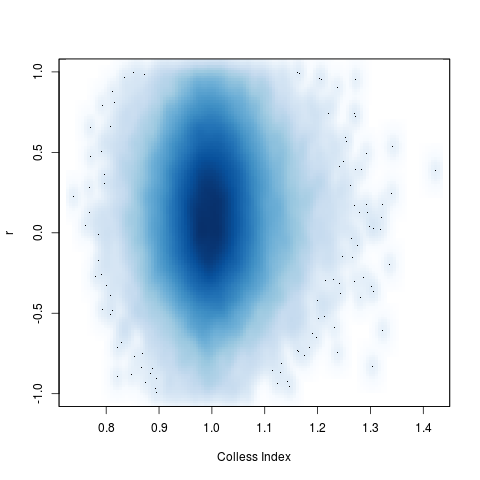
\includegraphics[width=.5\textwidth]{trueColless.png}
  \caption{\textbf{Effect of the True Colless Index of Full Phylogeny.}}
\end{figure}

\begin{figure}[!ht]
  \center
  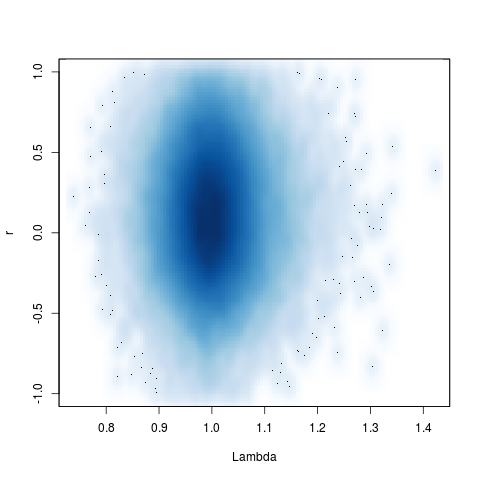
\includegraphics[width=.5\textwidth]{trueLambda.png}
  \caption{\textbf{Effect of the True Lambda of Full Phylogeny.}}
\end{figure}

\begin{figure}[!ht]
  \center
  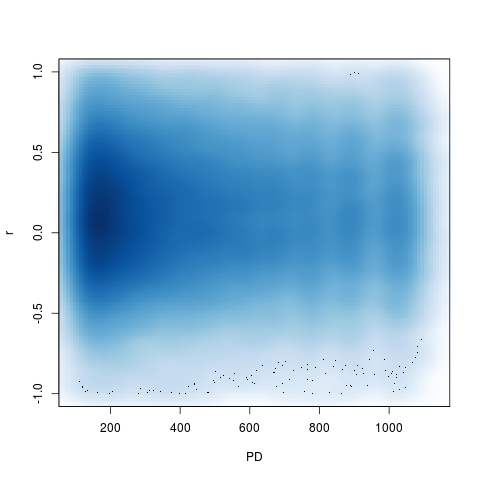
\includegraphics[width=.5\textwidth]{PD.png}
  \caption{\textbf{Effect of True PD of Full Phylogeny.}}
\end{figure}

\begin{figure}[!ht]
  \center
  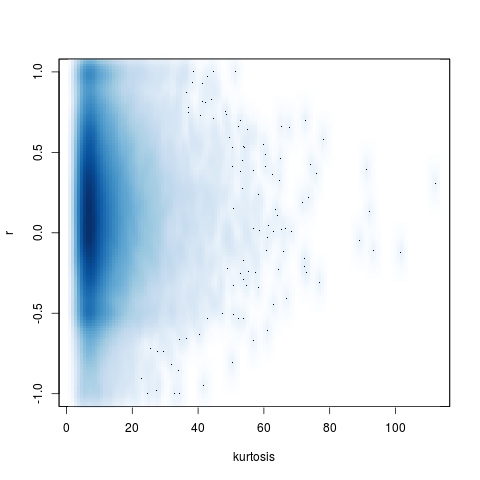
\includegraphics[width=.5\textwidth]{originalKurtosis.png}
  \caption{\textbf{Effect of the True Kurtosis of Full Phylogeny.}}
\end{figure}

\begin{figure}[!ht]
  \center
  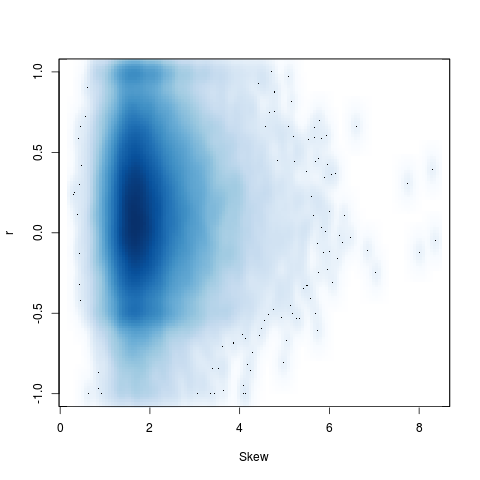
\includegraphics[width=.5\textwidth]{originalSkew.png}
  \caption{\textbf{Effect of the True Skew of Full Phylogeny.}}
\end{figure}

\clearpage
\section*{B. Error Rate in Top Rankings}

\begin{figure}[!ht]
  \center
  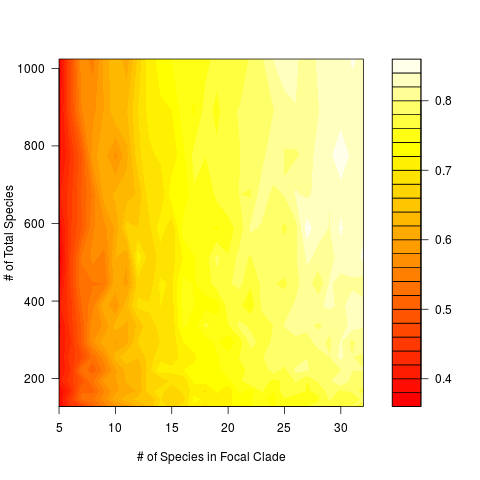
\includegraphics[width=.5\textwidth]{errorRate50.png}
  \caption{\textbf{Mean error rate in the ranking of top 50 species.}}
\end{figure}

\begin{figure}[!ht]
  \center
  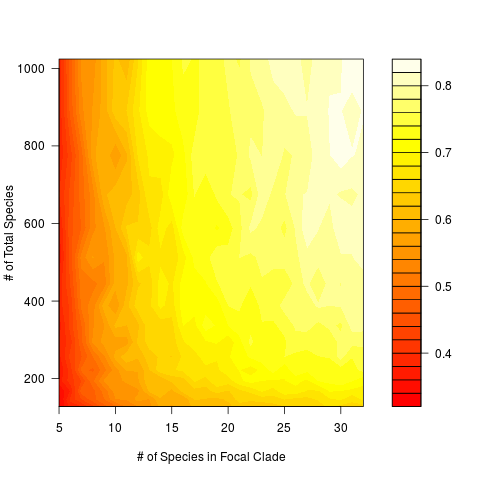
\includegraphics[width=.5\textwidth]{errorRate100.png}
  \caption{\textbf{Mean error rate in the ranking of top 100 species.} }
\end{figure}

\begin{figure}[!ht]
  \center
  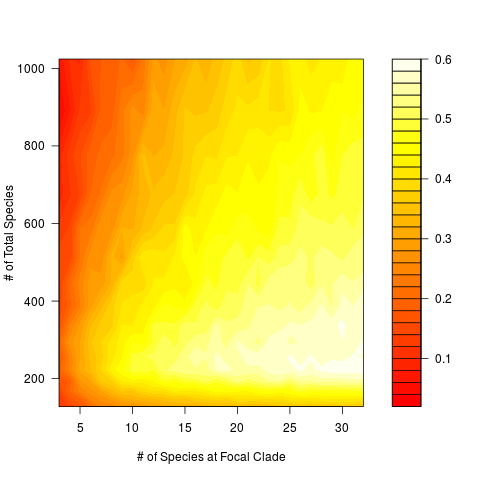
\includegraphics[width=.5\textwidth]{errorRate200.png}
  \caption{\textbf{Mean error rate in the ranking of top 200 species.} }
\end{figure}

\begin{figure}[!ht]
  \center
  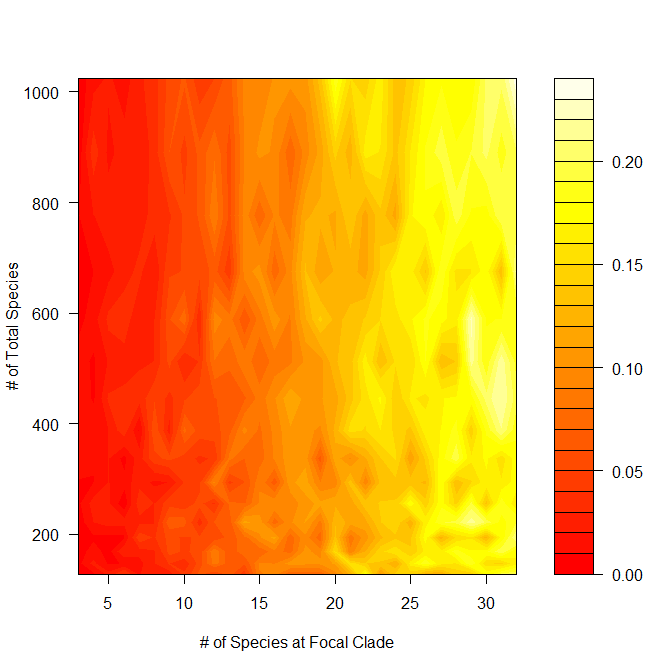
\includegraphics[width=.5\textwidth]{errorRate5pct.png}
  \caption{\textbf{Mean error rate in the ranking of top 5\% of species.} }
\end{figure}

\begin{figure}[!ht]
  \center
  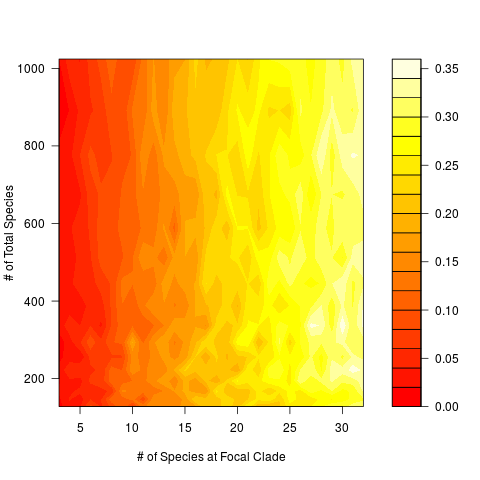
\includegraphics[width=.5\textwidth]{errorRate10pct.png}
  \caption{\textbf{Mean error rate in the ranking of top 10\% of species.} }
\end{figure}

\begin{figure}[!ht]
  \center
  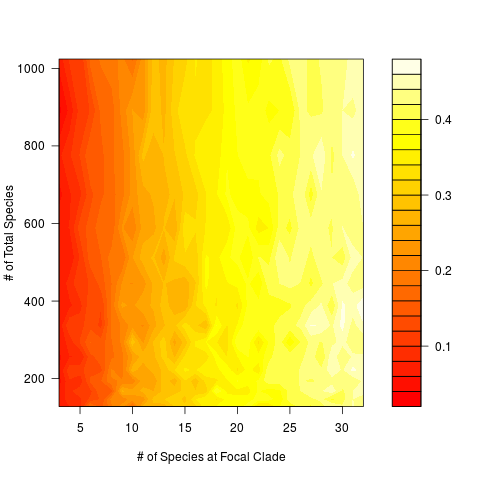
\includegraphics[width=.5\textwidth]{errorRate20pct.png}
  \caption{\textbf{Mean error rate in the ranking of top 20\% of species.}}
\end{figure}

\clearpage
\section*{C: Quantile regression of imputed correlations}
\begin{figure}[!ht]
  \center
  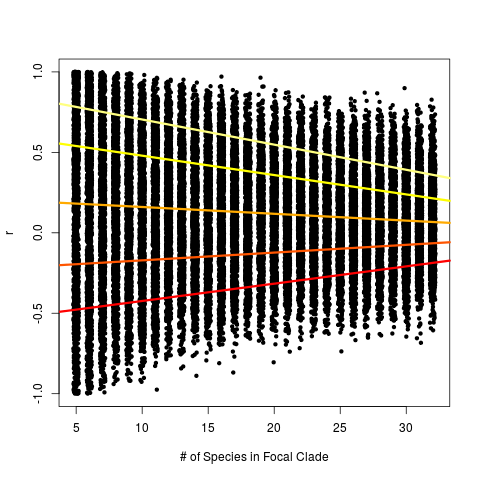
\includegraphics[width=.5\textwidth]{quantModel.png}
  \caption{\textbf{Quantile regression of r-values against size of imputed
  clades.} Each data point denotes a correlative comparison between ED values
  within the focal clades where imputation has occurred. Each regression line
  (top to bottom) represent quantile regressions from highest to lowest,
  respectively. Each of the regression lines demonstrate a convergence of the
  variation in r-values around zero.}
  \label{quantReg}
\end{figure}

\begin{table}[ht]
  \centering
  \begin{tabular}{rrrrrr} \hline
  & $\tau$ = 0.10 & $\tau$ = 0.25 & $\tau$ = 0.50 & $\tau$ = 0.75 & $\tau$ = 0.90 \\\hline
  (Intercept) & -0.54 & -0.23 & 0.20 & 0.60 & 0.86 \\
    Size of Focal Clade & 0.01 & 0.01 & -0.00 & -0.01 & -0.02 \\
    \hline
    \hline
  \end{tabular}
  \caption*{\textbf{Table 3: Quantile Regression of Clade Size and Total Species
  on Ranking Error.} Quantile regression model demonstrating the effect of clade
  size on the correlation between true and imputed ED values. The quantile
  regression estimates demonstrate statistical significance that as imputed
  clade size increases, variation in coefficient of correlation (r) between ED
  values center around zero (all p-values are $<$0.0001).}
\end{table}
\end{document}
%%% Local Variables:
%%% mode: latex
%%% TeX-master: t
%%% End:
